\loesung{}{
\begin{enumerate}[a)]
\item Inspect Implemented Functions

\lstinputlisting[firstline=1,lastline=84]{"rsrc/helper_functions_lime.R"}

Example: 
\lstinputlisting{"rsrc/data_lime.R"}
\lstinputlisting[firstline=6,lastline=11]{"rsrc/helper_functions_plot_lime.R"}

\begin{center}
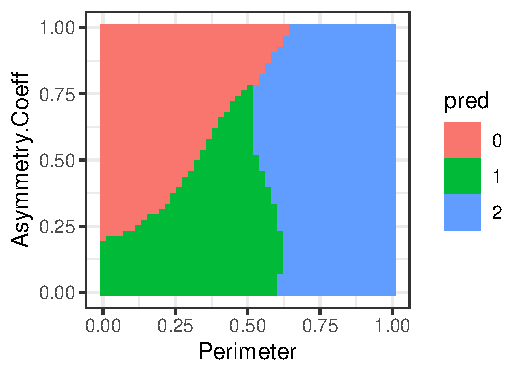
\includegraphics[width=\maxwidth]{figure/helper_functions_plot_lime.pdf}
\end{center}

\item Sample Points
\lstinputlisting[firstline=87,lastline=110]{"rsrc/helper_functions_lime.R"}

Example:
\lstinputlisting[firstline=5,lastline=9]{"rsrc/sample_points_plot_lime.R"}

\begin{center}
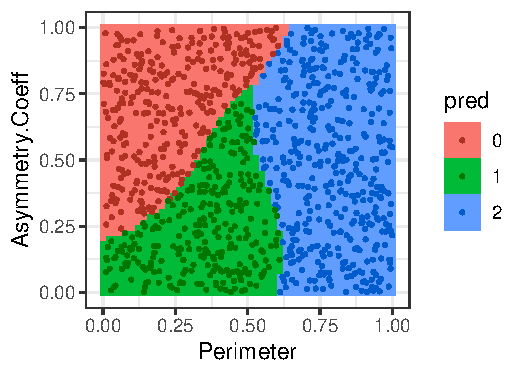
\includegraphics[width=\maxwidth]{figure/sample_points_plot_lime.pdf}
\end{center}

\item Weight Points
\lstinputlisting[firstline=114,lastline=140]{"rsrc/helper_functions_lime.R"}

Example:
\lstinputlisting[firstline=5,lastline=10]{"rsrc/weight_points_plot_lime.R"}

\begin{center}
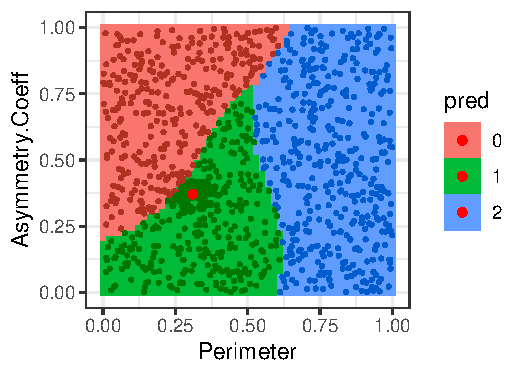
\includegraphics[width=\maxwidth]{figure/weight_points_plot_lime.pdf}
\end{center}

\item Fit Local Surrogate
\lstinputlisting[firstline=143,lastline=158]{"rsrc/helper_functions_lime.R"}

Example:
\lstinputlisting[firstline=5,lastline=22]{"rsrc/fit_explainer_model_plot_lime.R"}
\begin{center}
  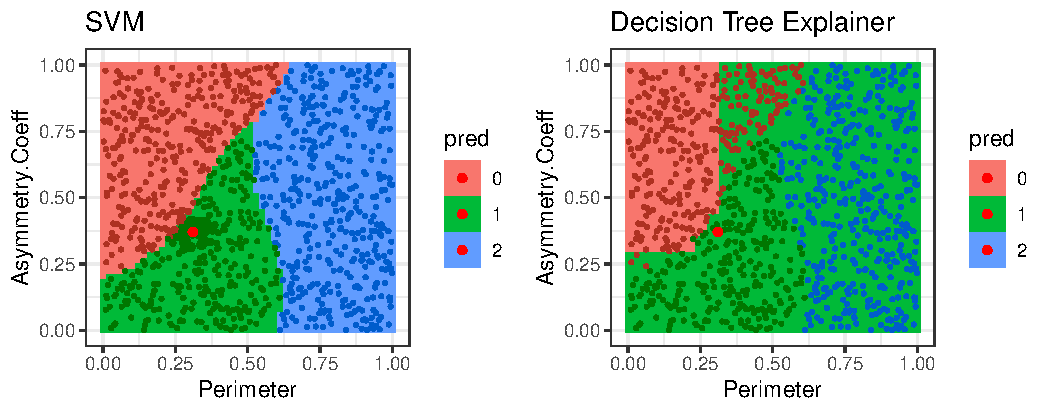
\includegraphics[width=\maxwidth]{figure/fit_explainer_model_plot_lime.pdf}
\end{center} 
  






\end{enumerate}
}